\section{Segment Anything Model} \label{sec:sam}

The Segment Anything Model (SAM) \cite{kirillov2023segany} is a state-of-the-art tool for image segmentation. It is designed as a general-purpose segmentation model that works across a wide range of images. However, the samples used in this work are very specific, and pixel-level precision is crucial.

As shown in Figure~\ref{fig:enter-label} and ~\ref{fig:sam}, even when using 5 positive and 9 negative points to guide the segmentation, SAM struggles to distinguish between the coating and the upper oxidation layer. This is not ideal, as researchers would need to manually place many guidance points for each measurement and still often need to refine the mask using a brush tool.

Another important limitation is the high hardware requirements of SAM. Unlike convolutional neural networks (CNNs), SAM is based on transformers, which are much more demanding in terms of computational resources. Since the measurements in this work are performed on standard computers, SAM is less practical.

Because of these challenges, the next method explored is based on CNNs.

\begin{figure} [H]
    \centering 
    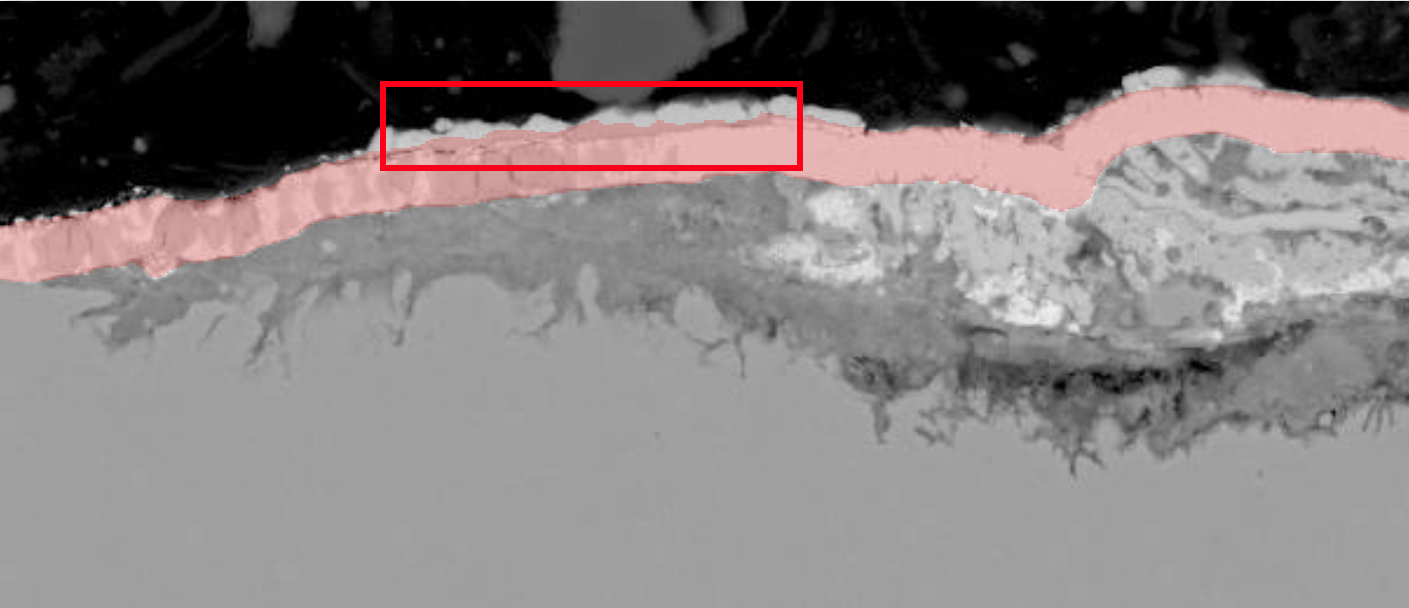
\includegraphics[width=0.7\linewidth]{PICTURES/SAM/rect.png} 
    \caption{Output mask generated by SAM. The red rectangle highlights the difficulty in distinguishing between the oxidation and coating layers.}

    \label{fig:sam} 
\end{figure}

\begin{figure} [H]
    \centering 
    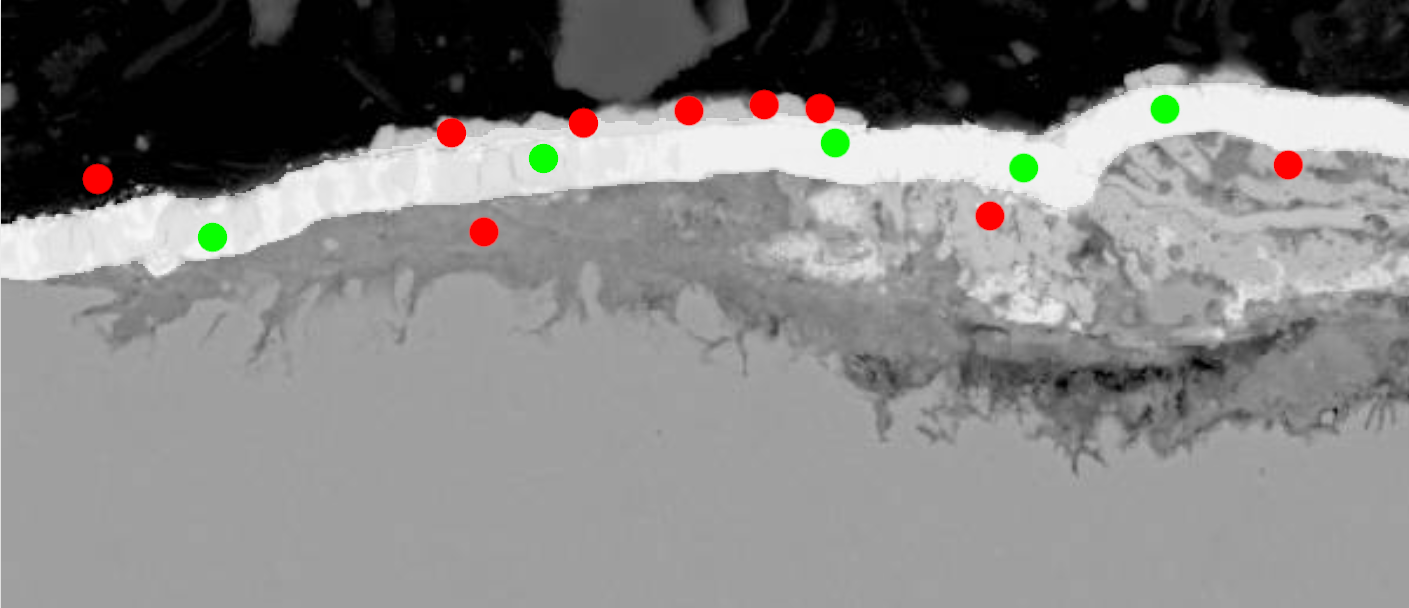
\includegraphics[width=0.7\linewidth]{PICTURES/SAM/points_sam.png} 
    \caption{User-provided positive (green) and negative (red) points used to guide the SAM segmentation.} \label{fig:enter-label} 
\end{figure}